\documentclass[notumble,combine]{leaflet}
%\documentclass[a4paper,notumble,combine,debug]{leaflet}
%\usepackage[utf8]{inputenc}
%\usepackage[T1]{fontenc}
%\usepackage{lmodern}
%\renewcommand{\bfdefault}{b}
%\usepackage{microtype}
\usepackage[dvipsnames,usenames]{color}
%\usepackage[dvipdfmx]{graphicx}
%\usepackage[dvipdfmx]{graphicx, color}
\usepackage{graphicx}
\usepackage{alltt}
\usepackage[dvipdfmx]{hyperref}
\usepackage{ascmac}
\usepackage{comment}
\usepackage{here}
\usepackage{wrapfig}
\usepackage{floatflt}
%\usepackage{ifthen}

\makeatletter
% Section color
%% from leaflet.cls
\renewcommand\section{\@startsection{section}{1}{\z@}%
  {-3.5ex \@plus -.75ex}%
  {1ex} %{1.5ex}%
  {\normalfont\Large\sectfont\color{NavyBlue}\addul}}
\newcommand{\addul}[1]{\underline{#1}}
\renewcommand\subsection{\@startsection{subsection}{2}{\z@}%
  {-2.5ex plus -.5ex}%
  {1\p@} %{1ex}%
  {\normalfont\large\sectfont\color{Green}\addul}}
  \renewcommand\subsubsection{\@startsection{subsubsection}{2}{\z@}%
  {-1.5ex plus -.25ex}%
  {0.5\p@} %{1ex}%
  {\normalfont\normalsize\sectfont\color{Emerald}\addul}}
  \makeatother

\graphicspath{{figures/}} 

\title{
	\resizebox{\linewidth}{!}{\bf\color{Orange} スタックチャン}\\
	\vfill
	\parbox[c]{\textwidth}{
\includegraphics[width=\textwidth]{img/stackchan.eps}}\\
%	[\baselineskip]
	\vfill
  \resizebox{\linewidth}{!}{\bf \color{Red} コミュニケーションロボットをあなたの手に。}\\
  \resizebox{\linewidth}{!}{\bf \color{Red} スタックチャンはなにをしなくても、スーパーかわいい}\\
        \vfill
	\resizebox{\linewidth}{!}{\bf \href{https://scrapbox.io/stack-chan/}{スタックチャンコミュニティ}}\\
        \hfill {
\includegraphics[width=2cm]{img/Stackchan_flyer.eps}}\\
}



\date{2025年1月25日(土)版}
%\CutLine*{1} \CutLine*{2} \CutLine*{3} \CutLine*{4} \CutLine*{5}
%\CutLine*{6}

% \AddToBackground*{2}{% Background of a large page
%   \put(\LenToUnit{.25\paperwidth},\LenToUnit{.4\paperheight}){%
%     \includegraphics[width=14.85cm]{kbug-logo}
% }}

\hypersetup{
setpagesize=false,
 bookmarksnumbered=true,
 bookmarksopen=true,
 colorlinks=true,
 linkcolor=blue,
 citecolor=red,
}

\begin{document}
\maketitle
\thispagestyle{empty}
\pagebreak{}
\section{スタックチャンってなぁに?}
スタックチャンはししかわさんが開発、公開している、 手乗りサイズのスーパーカワイイコミュニケーションロボットです。 
作品ページ:https://github.com/meganetaaan/stack-chan

キャッチフレーズは、以下の通りです。
\begin{itemize}
  \item \resizebox{\linewidth}{!}{\bf\color{Red}コミュニケーションロボットをあなたの手に。}
  \item \resizebox{\linewidth}{!}{\bf\color{Red}スタックチャンはなにをしなくても、スーパーかわいい}
\end{itemize}

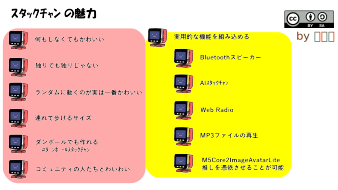
\includegraphics[width=\textwidth]{img/stackchan-salespoint.eps}

\section{スタックチャンのはじめかた}
\subsection{M5Stackの選び方}
M5Stackは、これらを選ぶと良いと思います。
\begin{itemize}
  \item Core2 or Core2 aws: 色々試したければこれ。
  \item Atom Echo: AIスタックチャンミニマルならこれ。
\end{itemize}

\subsection{お顔だけでも楽しいですよ!!}
スタックチャンの多くのプログラムは、体がなくてもM5Stack単体だけで動作します。
たくさんのプログラムが、M5Stack用のプログラム書き込みツールM5Burnerで提供されています。


\subsection{動かすにはなにを用意したらいいの?}
動くスタックチャンを作るためには、以下のものが必要です。

\begin{itemize}
  \item M5Stack本体
  \item 3Dプリンタで作った筐体
  \item サーボモータと専用基板
\end{itemize}

\subsection{あなたはどのスタックチャン?}
スタックチャンを作成するには、いくつかの選択肢があります。
例えば、M5Stackになにを選ぶのか、筐体をどうするか、サーボモータにどんなものを使うのか、などです。

\section{スタックチャン3つのオープン}
スタックチャンは、以下の3つのオープンな環境です。
\begin{itemize}
  \item オープンな仕様
  \item オープンなプロセス
  \item オープンなコミュニティ
\end{itemize}

では、各項目を詳しく見ていきましょう。

\subsection{オープンな仕様}
普通の意味でのオープンソースです。

スタックチャンは、ソフトウエアがオープンになっています。
AIやBluetoothスピーカーなどのバージョンのスタックチャンのソースが公開されています。

ハードウエアもオープンになっています。
ハードウエアには、以下のようなものがあります。
\begin{itemize}
  \item 筐体データ(3Dプリント)がオープン
  \item 基板の設計データがオープン
\end{itemize}

\subsection{オープンなプロセス}
スタックチャンは、 制作の過程もオープンになっています。

制作の過程がオープンとは、DiscordやXでスタックチャンの制作例が多数報告されており、自分で製作する時の参考情報が多数手に入ることを意味しています。
ここでは、成功例が手に入るだけでなく、失敗例も手に入るようになっています。

スタックチャンのオープンなプロセスでは、難しいことを難しいと言える雰囲気を大事にしています。


\subsection{オープンなコミュニティ}
 スタックチャンコミュニティは誰にでもひらかれています。

スタックチャンコミュニティでは、全員がユーザーであり開発者でもあります。

うちの子自慢も盛んに行われていますので、あなたのスタックチャン自慢も是非してみてください。

手芸やキーホルダーなどのアクセサリで参加している人たちもいます。

最近は、もくもく会やオンリーイベントなども行われています。
詳しくは、イベント情報をご覧ください。

\newpage
\section{色々なスタックチャン}
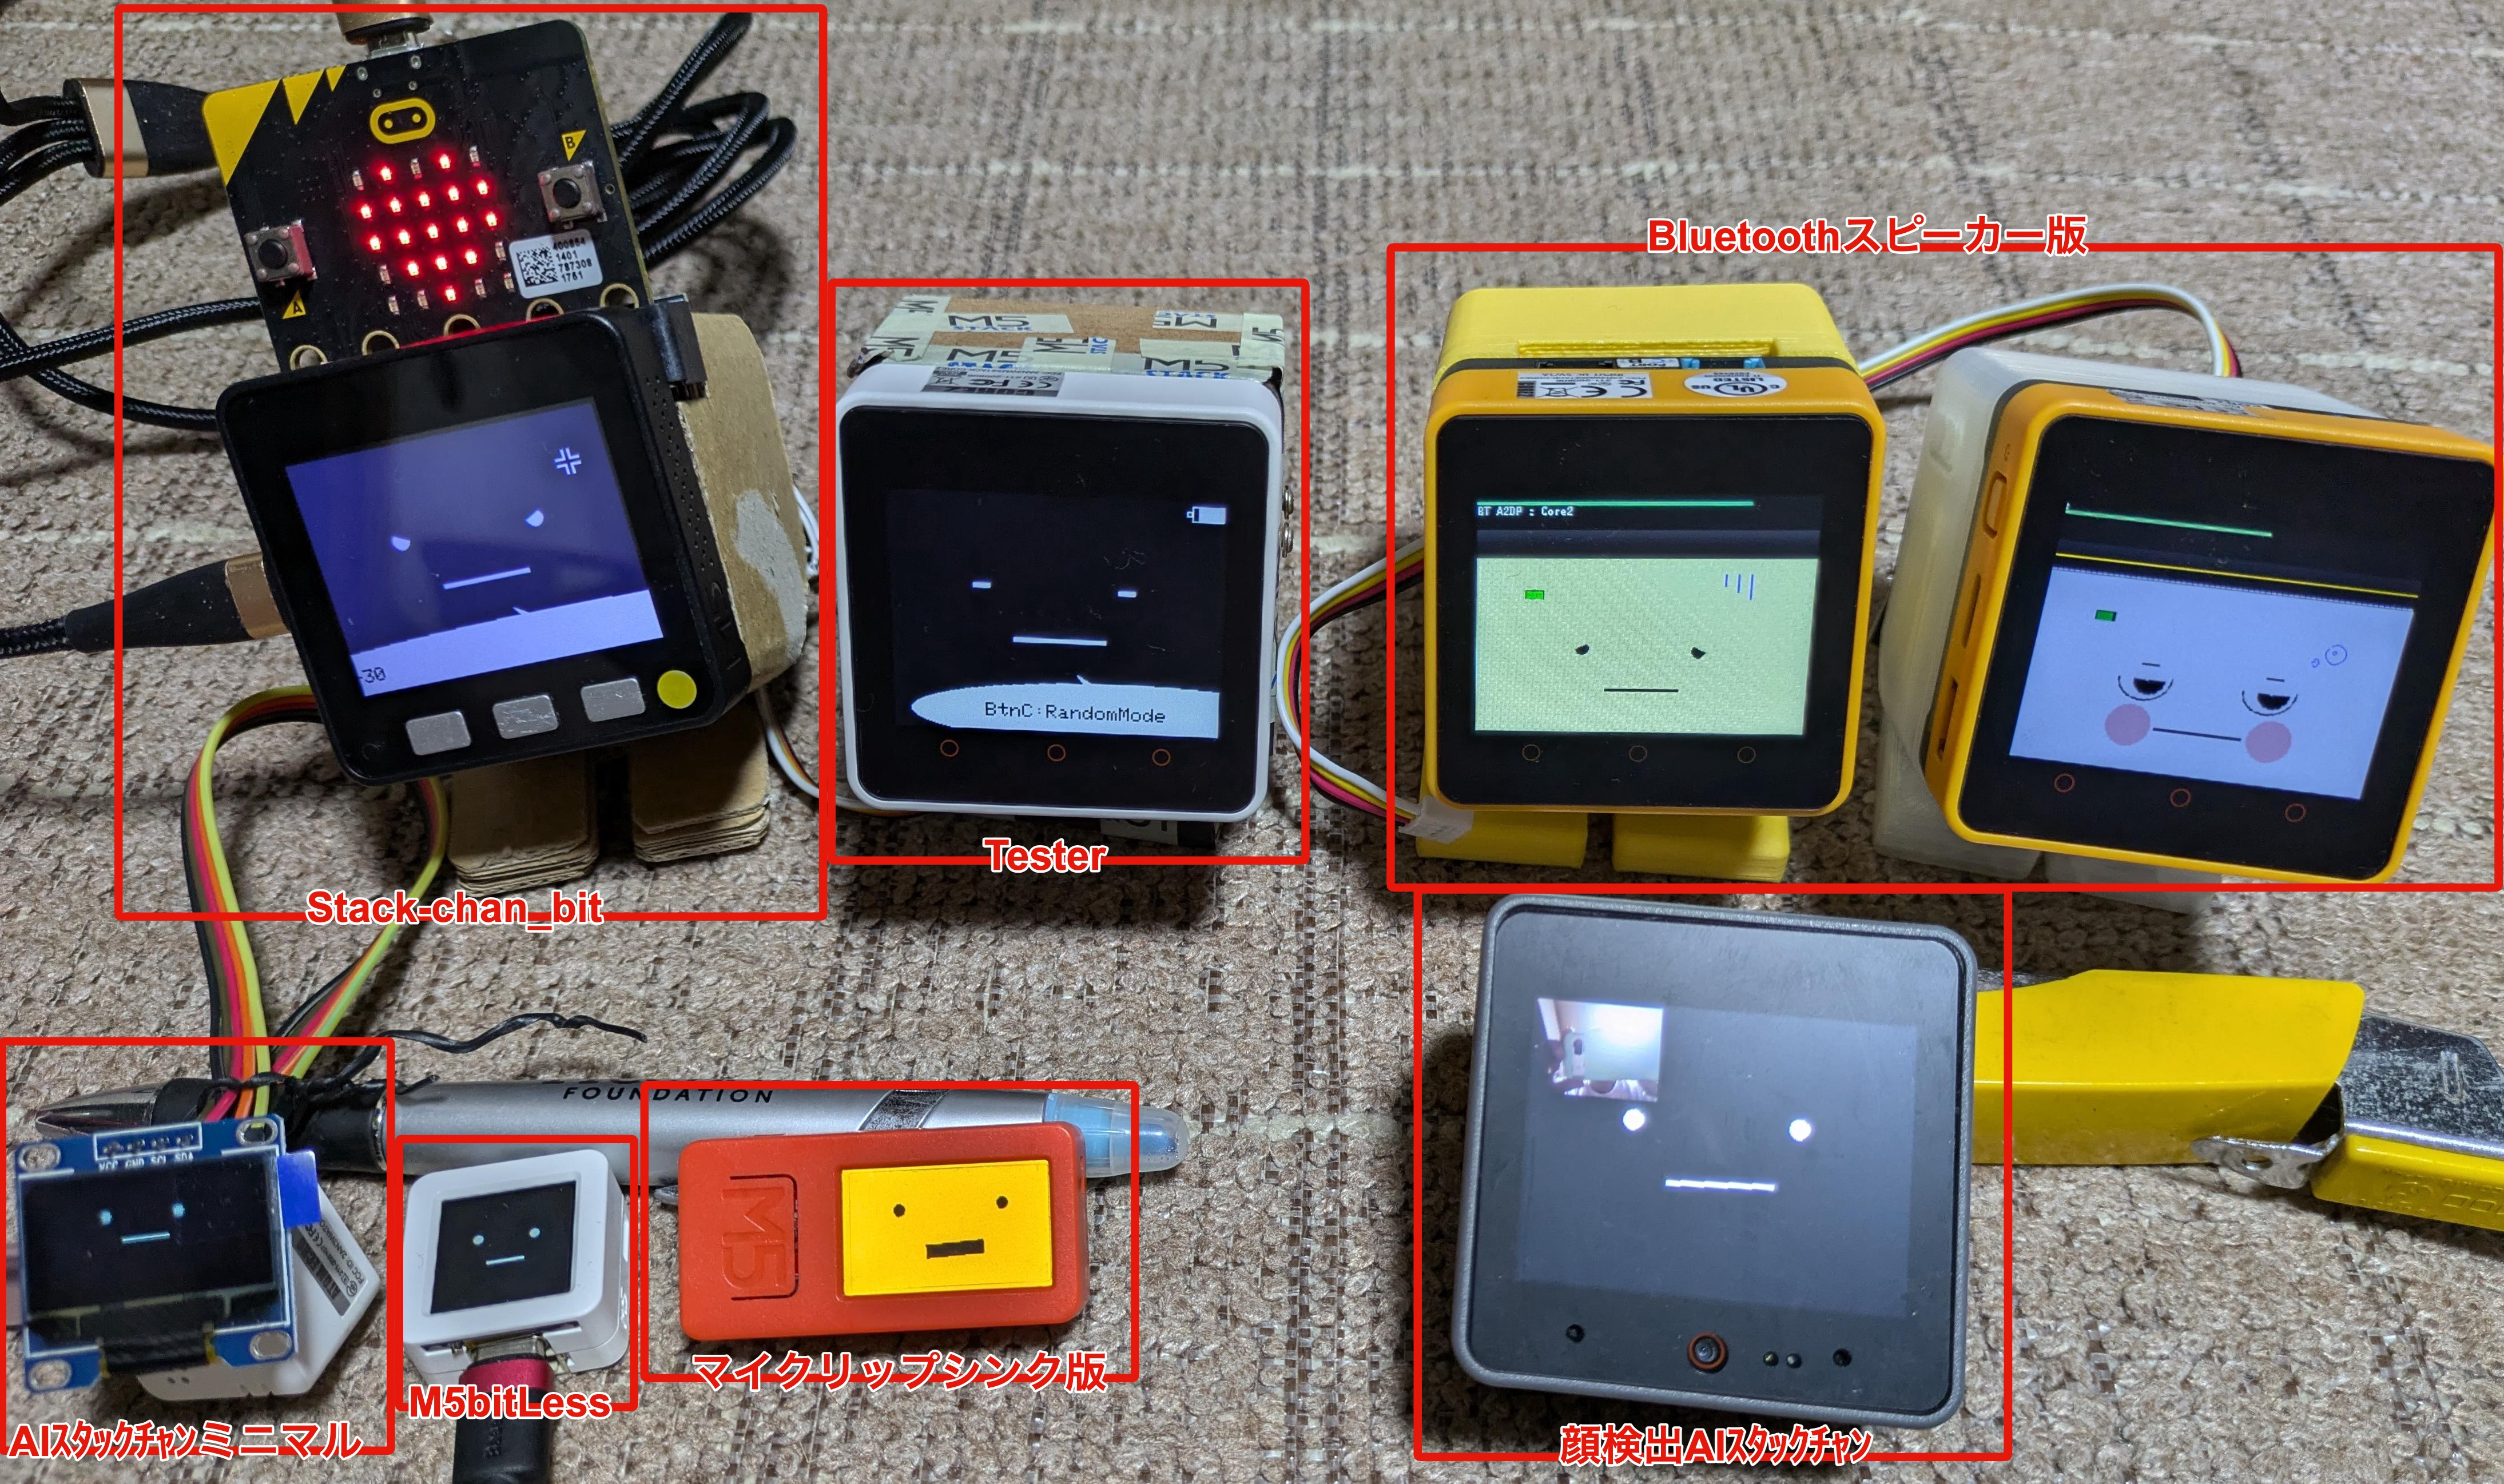
\includegraphics[width=\textwidth]{img/stackchans.eps}

スタックチャンには色々な種類のものがあります。
\begin{itemize}
  \item Bluetoothスピーカー版:リップシンクしてくれます
  \item AI版:音声入出力でAIエージェントとして動きます
  \item Radiko版:Radikoが聴けます
  \item 時計版:時計にもなります
  \item Stack-chan\_bit版:microbitとも使えます
  \item 動作テスター版:初期設定用です
\end{itemize}

\subsection{Bluetoothスピーカー版}
スタックチャンがBluetoohスピーカーとして動作し、音に合わせてリップシンクしてくれます。
まるで、スタックチャンがしゃべっているようです!!

\subsection{AI版}
AI版スタックチャンは、スタックチャンがAIとして動作するバージョンです。
スタックチャンが音声で質問を聞いてくれ、ChatGPTなどのAIに問い合わせ、答えを音声で教えてくれます。

\subsubsection{顔検出版CoreS3用AIスタックチャン}
CoreS3にはカメラがあり、これで顔検出してAI動作をしてくれます。

\subsubsection{AIスタックチャンミニマル}
AIスタックチャンミニマルは、誰にでも気軽にスタックチャンが楽しめるようにというコンセプトで作られたバージョンです。
5000円程度で作ることができます。

\newpage
\section{関連イベント(予定)}
\begin{itemize} 
  \item 2025/01/25: OSC 2025 Osakaブース展示 \& LT(オープンソースとスタックチャン)
  \item 2025/02/01: 東京もくもく会@赤坂 オンライン配信あり
  \item 2025/02/15: 神奈川もくもく会@関内 オンライン配信あり
  \item 2025/04/05: スタックチャンオンリーイベント@\href{https://extinct-media-museum.blog.jp/otemachi/}{絶滅メディア博物館}(東京)
  \item 未定(日程調整中): 大阪もくもく会@\href{https://www.r3it.com/ashibinaa}{gusuku Ashibinna Osaka}(グランフロント大阪)
  \item 未定(7/2前後?): スタックチャン4歳のお誕生日会2025
\end{itemize}

\vfill
\begin{minipage}{\textwidth}
\begin{boxnote}

\section{スタックチャン情報}
スタックチャンに関する情報は、以下のような場所で入手することができます。

\begin{itemize}
  \item \href{https://scrapbox.io/stack-chan/}{Cosense:情報集約用}
  \item \href{https://discord.gg/eGhd9adnBm}{Dicsord}
  \item X:
	\href{https://x.com/stack_chan}{@stack\_chan}
	ハッシュタグ:\href{https://x.com/search?q=%23%EF%BD%BD%EF%BE%80%EF%BD%AF%EF%BD%B8%EF%BE%81%EF%BD%AC%EF%BE%9D&src=typed_query&f=live}{\#スタックチャン}
  \item mixi2:スタックチャンコミュニティ
  \item ProtoPedia:プロトタイプ投稿サイト\url{https://protopedia.net/material/833}
\end{itemize}


\includegraphics[width=2.2cm]{img/cosense.eps}

\includegraphics[width=2.2cm]{img/discord.eps}

\includegraphics[width=2.2cm]{img/X.eps}

\end{boxnote}
\end{minipage}
\end{document}
